\documentclass[tikz,border=3pt]{standalone}
\usepackage[utf8]{inputenc}
\usepackage[T1]{fontenc}
\usepackage{lmodern}
\renewcommand{\familydefault}{\sfdefault}
\usepackage{sansmath}\sansmath
\usepackage{chemfig}
\usepackage{pgfplots}\pgfplotsset{compat=1.18,/pgf/number format/use comma,/pgf/number format/1000 sep={.}}
\usetikzlibrary{arrows.meta,calc,positioning,decorations.pathmorphing,patterns}
% paleta del sitio
\definecolor{nar}{HTML}{E8680C}\definecolor{narc}{HTML}{FFB35C}\definecolor{hielo}{HTML}{FFF3E8}
\definecolor{tinta}{HTML}{1D1D1F}\definecolor{gris}{HTML}{6E6E73}\definecolor{lila}{HTML}{7C5CF0}
\definecolor{azul}{HTML}{2F6FD6}\definecolor{menta}{HTML}{17A673}\definecolor{coral}{HTML}{E8342A}
\begin{document}
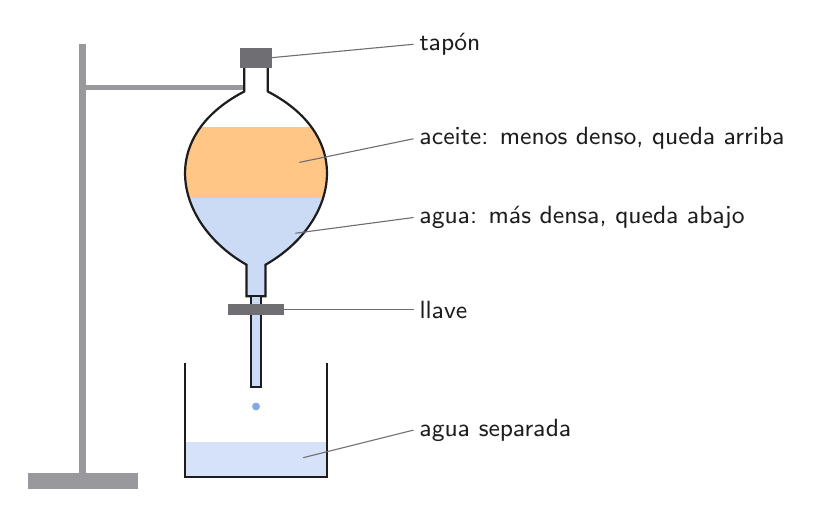
\begin{tikzpicture}[font=\small]

\fill[gris!70] (-2.9,-0.15) rectangle (-1.5,0.05);
\draw[gris!70,line width=2.5pt] (-2.2,0.05) -- (-2.2,5.5);

\draw[gris!70,line width=1.6pt] (-2.2,4.95) -- (-0.17,4.95);
\fill[azul!20] (-0.9,0) rectangle (0.9,0.45);
\draw[tinta,thick] (-0.9,1.45) -- (-0.9,0) -- (0.9,0) -- (0.9,1.45);
\begin{scope}\clip (-0.15,5.2) -- (-0.15,4.9) .. controls (-1.3,4.3) and (-1.0,3.2) .. (-0.12,2.7) -- (-0.12,2.3) -- (0.12,2.3) -- (0.12,2.7) .. controls (1.0,3.2) and (1.3,4.3) .. (0.15,4.9) -- (0.15,5.2) -- cycle;
\fill[white] (-2,2) rectangle (2,5.3);
\fill[azul!25] (-2,2) rectangle (2,3.55);
\fill[narc!75] (-2,3.55) rectangle (2,4.45);
\end{scope}
\draw[tinta,thick] (-0.15,5.2) -- (-0.15,4.9) .. controls (-1.3,4.3) and (-1.0,3.2) .. (-0.12,2.7) -- (-0.12,2.3) -- (0.12,2.3) -- (0.12,2.7) .. controls (1.0,3.2) and (1.3,4.3) .. (0.15,4.9) -- (0.15,5.2);
\draw[tinta,thick,fill=azul!25] (-0.06,2.3) rectangle (0.06,1.15);
\fill[gris] (-0.36,2.06) rectangle (0.36,2.2);
\fill[gris] (-0.2,5.2) rectangle (0.2,5.45);
\fill[azul!60] (0,0.9) circle (0.05);
\draw[gris] (0.2,5.33) -- (2,5.5) node[anchor=west,text=tinta,align=left,inner sep=2pt] {tapón};
\draw[gris] (0.55,4) -- (2,4.3) node[anchor=west,text=tinta,align=left,inner sep=2pt] {aceite: menos denso, queda arriba};
\draw[gris] (0.5,3.1) -- (2,3.3) node[anchor=west,text=tinta,align=left,inner sep=2pt] {agua: más densa, queda abajo};
\draw[gris] (0.36,2.13) -- (2,2.13) node[anchor=west,text=tinta,align=left,inner sep=2pt] {llave};
\draw[gris] (0.6,0.25) -- (2,0.6) node[anchor=west,text=tinta,align=left,inner sep=2pt] {agua separada};

\end{tikzpicture}
\end{document}
